\section{Five-dimensional estimator: validation and uncertainty}
\label{sec:5d}

This section validates the five-dimensional estimator behind the central values of \S\S\ref{sec:3d}--\ref{sec:eavailw}. It covers what each test isolates (\S\ref{sec:val-fiveaxis}), background subtraction and generator-sized truth changes (\S\ref{sec:val-negweight}), why the estimator does not follow such changes (\S\ref{sec:val-departure}), model dependence and the reporting definitions it rules out (\S\ref{sec:gbdt-model-dependence}), the coverage test (\S\ref{sec:coverage-5d}) and the status of the five-axis covariance of the configuration-(a) central value (\S\ref{sec:eavailw-construction}). The sixteen-cell result of configuration (e) follows in \S\ref{sec:fived16}, and the calibrated generator tests built on a variant of this estimator in \S\ref{sec:joint5d}. The unbinned negative-weight background method itself is derived in App.~\ref{app:negweight}.

\subsection{Which source of error is being tested}
\label{sec:val-fiveaxis}
Prior reweighting changes the frequencies of existing simulated truth events while retaining their detector-response simulation; a response mismatch instead changes how a given truth is reconstructed. Finite classifier capacity and iteration count approximate the inverse and can leave residuals in either case. Coverage asks whether the resulting intervals contain their specified target at the stated rate (\S\ref{sec:coverage-5d}). These mechanisms are separate: an incorrect generator prediction alone does not diagnose an interval failure. Each test below isolates one intervention.
% Register round n1 (R-N1): the two findings summarized here print at their homes: the refined subtraction's nominal
% recovery in sec:val-negweight and sec:val-departure, and the signal-only result in sec:val-negweight.


All 2D closures in \S\ref{sec:validation} unfold reweighted simulated signal without background, so they do not test background subtraction.

% Methods-paper shortening pass (2026-10-21, DECISION-20261020-joseph-refined-estimator-shorten-delta.md item 2): the article's validation-design table, moved with its sources: 3D/4D closure, sec_validation.tex (thresholds); background closure OUTCOME-20260925-s5c-purity- background-bias-at-high-W.md:1-10 and s5n stage 1; generator-sized change, this section ("predeclared GiBUU-to-GENIE departure screen"); withheld shapes, OUTCOME-20260926-s5e-oi192-diagnosis-and-candidate.md (A4, compared with the adopted sigma); coverage, OUTCOME-20260925-s5c-tier-s-futility-fail.md:30-36; calibration, amendment 7 and sec_joint.tex. REVIEW-1 finding 2: no record that the 3D threshold was set in advance (sec_validation.tex:138-144). The tilt: truth weight 1 + 0.2 (u - 1/2), u = E_avail/100 GeV (nd-unfolding/s5c_pseudo.py:67-70); KNOWN_ISSUES row 98.
\providecommand{\pcell}[2]{\parbox[t]{#1}{\raggedright\strut#2\strut}}
Table~\ref{tab:validation-design-5d} lists the validation studies of the article and of this note (detector response: \S\ref{sec:closure-map} and \S\ref{sec:joint5d-calibration}). Letters refer to Table~\ref{tab:estimators-matrix}.

\begin{table}[htbp]
  \caption{Validation studies of the article and of this note.}
  \label{tab:validation-design-5d}
  \centering\footnotesize
  \begin{tabular}{@{}lllll@{}}
    \toprule
    \pcell{0.17\textwidth}{Study} & \pcell{0.22\textwidth}{Truth change} & \pcell{0.10\textwidth}{Backgrounds} &
    \pcell{0.16\textwidth}{Domain} & \pcell{0.23\textwidth}{Criterion} \\
    \midrule
    \pcell{0.17\textwidth}{Two-dimensional reproduction (f), (a), (b)} & \pcell{0.22\textwidth}{none: data against the publication} &
    \pcell{0.10\textwidth}{data} & \pcell{0.16\textwidth}{205 published bins} & \pcell{0.23\textwidth}{none; descriptive} \\
    \pcell{0.17\textwidth}{Three-, four-observable closure (a)} & \pcell{0.22\textwidth}{injected bump in truth $\Eavail$ (three observables) or $q_{3}$ (four)} &
    \pcell{0.10\textwidth}{none} & \pcell{0.16\textwidth}{one-dimensional marginals} & \pcell{0.23\textwidth}{descriptive: residual ratio 0.10 ($\Eavail$; \S\ref{sec:3d-closure}, \S\ref{sec:closure-map})} \\
    \pcell{0.17\textwidth}{Background closure (c), (d)} & \pcell{0.22\textwidth}{none (nominal truth)} &
    \pcell{0.10\textwidth}{included} & \pcell{0.16\textwidth}{42 $(\Eavail,W)$ and \jtNcells{} joint cells} & \pcell{0.23\textwidth}{none; studies during estimator development} \\
    \pcell{0.17\textwidth}{Generator-sized change (d)} & \pcell{0.22\textwidth}{GiBUU/GENIE $\Eavail$ shape ratio} &
    \pcell{0.10\textwidth}{included} & \pcell{0.16\textwidth}{42 $(\Eavail,W)$ cells} & \pcell{0.23\textwidth}{recovery requirement; not met} \\
    \pcell{0.17\textwidth}{Shapes held out of development (e)} & \pcell{0.22\textwidth}{NuWro and GENIE + MEC shapes, not used while (e) was chosen} &
    \pcell{0.10\textwidth}{included} & \pcell{0.16\textwidth}{42 $(\Eavail,W)$ cells} & \pcell{0.23\textwidth}{compared with the configuration-(a) total $\sigma$} \\
    \pcell{0.17\textwidth}{Coverage (c)} & \pcell{0.22\textwidth}{nominal; signal rate lowered by about 10\% with a weak $\Eavail$ slope (weight 0.900--0.906 below \SI{3}{GeV})} &
    \pcell{0.10\textwidth}{included} & \pcell{0.16\textwidth}{153 cell and projection integrals} & \pcell{0.23\textwidth}{upper bound on coverage at least 0.66 (0.94)} \\
    \pcell{0.17\textwidth}{Test calibration (e)} & \pcell{0.22\textwidth}{each null hypothesis} &
    \pcell{0.10\textwidth}{included} & \pcell{0.16\textwidth}{\jtNcells{} (GiBUU \jtNcellsGiBUU) joint cells} & \pcell{0.23\textwidth}{size set by the calibration (\S\ref{sec:joint5d-frozen})} \\
    \bottomrule
  \end{tabular}
\end{table}

\subsection{Background subtraction and generator-sized truth changes}
\label{sec:val-negweight}

\paragraph{Background subtraction.}

End-to-end five-dimensional pseudo-experiments add background-simulation events and rebuild per-bin purity weights as in the measurement. At nominal truth they return the highest-$W$ column of $(\Eavail,W)$ \SIrange{3.5}{4.1}{\percent} low and the highest-$\Eavail$, highest-$W$ cell \SI{1.7}{\percent} high; without background, the same experiments recover the truth to \SI{0.22}{\percent}. Relative to these cells' total uncertainty in the configuration-(a) covariance, the bias is 0.36--1.07 standard deviations. The bias comes from the purity-based subtraction (\S\ref{app:negweight}), enters no quoted covariance, and has no established size on data. Refined unbinned negative-weight subtraction (App.~\ref{app:negweight}), applied with a deterministic variant of the five-dimensional LightGBM production estimator, brings the highest-$W$ column to \SIrange{0.11}{0.24}{\percent} and the corner cell to \SI{0.24}{\percent} over sixty nominal-truth experiments. Some joint cells remain up to \SI{1.0}{\percent} high, up to 14 standard errors, against \SI{-0.2}{\percent} without background; the mechanism is not established. On data, the two treatments differ by a median of \SI{0.36}{\percent} and at most \SI{1.4}{\percent} over the reported functionals. These differences measure method sensitivity, not bias. Negative-weight subtraction is not used for the configuration-(a) five-dimensional central value; the sixteen-cell result uses it (\S\ref{sec:fived16}).
% (scalar-5D campaign, development study D1)
% Sources: docs/orchestration/OUTCOME-20260925-s5c-purity-background-bias-at-high-W.md,
% docs/orchestration/state/s5c/d1/d1_summary.json, docs/orchestration/state/s5c/d1/bias_vs_adopted.json.
% CLI form: \texttt{-{}-bkg-mode negweight-refined}. Implementation (refinement to
% non-negative weights before the first OmniFold step; injection and independent
% subtraction halves of the background simulation) is in the negative-weight appendix (app:negweight).

\paragraph{Generator-sized truth changes.}

The unfolding does not follow a GiBUU-to-GENIE $\Eavail$ shape reweighting of the truth (0.70--1.33 per $\Eavail$ bin, total preserved). The GENIE prediction behind the ratio uses a mis-sampled flux (\S\ref{sec:3d-models}), so the ratio is a valid known-truth deformation of generator size but not a measured GiBUU--GENIE difference. The $(\Eavail,W)$ residuals have a median of \SI{9.7}{\percent}; they reach \SI{74}{\percent} in the highest-$W$ column and several percent in the largest cells. The \SI{74}{\percent} residual is in the cell $0.8\le\Eavail<\SI{1.5}{GeV}$, $W\ge\SI{3}{GeV}$, whose share of the cross section the deformation study did not record. A $q_3$ deformation preserving the $(\Eavail,W)$ truth shifts these cells by up to \SI{37}{\percent}. Signal-only experiments with the same seeds reproduce both results. The residuals are therefore a property of the estimator (five iterations, the GBDT configuration of \S\ref{sec:method}), not of the background treatment; their status in the quoted uncertainties is given in \S\ref{sec:val-departure}.
% KNOWN_ISSUES.md row 83
% Register round r12 (2026-10-21): the cell and the unrecorded share moved from the article's Sec. V B; source
% figures/methods_m3/fig_m3_deformation.py numbers output (EW29); dev_receipt.json and truth_check.json carry no yields.
% Register round n1 (R-N1): the status of this bias (it enters no quoted uncertainty) is stated once, at its home in
% sec:val-departure.
% Source: docs/orchestration/OUTCOME-20260925-s5n-stage1-development-fail.md (VL151, VL152);
% KNOWN_ISSUES 75, 77; independently reproduced (state/s5n/stage1/review-round-1.md).

\subsection{Why the estimator does not follow a generator-sized change}
\label{sec:val-departure}
% An instrumented rerun recorded every OmniFold iteration of these experiments. It reproduced the development results bitwise and repeated them through the unmodified driver, which shows the same response to the $\Eavail$ departure (highest-$W$ cell
% \SI{73.8}{\percent} against \SI{73.5}{\percent}).

Both OmniFold steps behave as intended: the first matches the reconstructed pseudo-data within statistical noise, and the second reproduces the truth-level weight sums to \SI{0.5}{\percent}. Yet the unfolded result folds back onto the data less well than the true model does. With noise-free pseudo-data the unfolding recovers more than \SI{99}{\percent} of the change that the departure produces in the reconstructed distribution, whereas the median $(\Eavail,W)$ truth residual ranges from \SI{5}{\percent} to \SI{11}{\percent}, with \SI{74}{\percent} in the worst cell. The unrecovered reconstructed-level difference is small relative to the departure but statistically significant at the analysis exposure.

With noise-free pseudo-data, thirty iterations reduce the $\Eavail$ residual by \SI{26}{\percent}; the $\Eavail$ residual continues to fall slowly, while the $q_3$ residual grows with iterations. A larger classifier improves the reconstructed-level fit without reducing the $\Eavail$ truth residual, and removing the regression for events that fail reconstruction does not reduce that residual either. No single cause is established, and no estimator change within the scope of the study meets the recovery requirement, set before the test, for the GiBUU-to-GENIE departure. The $\Eavail$ and $q_3$ residuals, a regularization (unfolding-model) bias of the estimator, enter no uncertainty quoted for the configuration-(a) central value. For the sixteen-cell result (\S\ref{sec:fived16}), the model term of the reported covariance is the change in the unfolded data when the prior is reweighted to each generator (GENIE + MEC, NuWro, GiBUU; \S\ref{sec:fived16-cov}). This term is unscaled and is not a calibrated bound. The fake-data study of \S\ref{sec:fived16-fd} measures the estimator's bias and compares it with the reported covariance.
% Register round n1 (R-N1, R-N6): the home of the residual-bias statement (moved from sec:val-negweight); "that the
% study's rules allow" stated as its scope (OUTCOME-20260926-s5e-oi192-diagnosis-and-candidate.md:43, "no authorized
% estimator change passes its predeclared screen").

% CLAIM-ADDITION D-ID BEGIN Register round 2 (methods paper, 2026-10-21), claim addition for Joseph, to be committed separately. Source: docs/orchestration/state/next-preparation-20261009/d-id/REPORT.md (simulation-only; NOT CITABLE FOR a coverage result or an interval, :7-13). Setting: T2, same-sample, nominal-weighted, K = 5, pooled over GiBUU (= D1), W1, W3, q3 and W2 (:394); the IBU starts from the nominal prior (:74) with exact efficiency (:183-186); reco binning 10,499 cells (:97, :382); W2's comparator is background-inclusive and the outcome is unchanged without it (:398, :204-207, :559). J medians at K = 5 (:432-440). Eligible 144, approximation-dominated 15, 2 identified, A share 0.014 (:398, :430-431, :530-532). C-counted 121 of 144, CR widths > 10% at both truth resolutions, median 31% at T1 = the J cells (:70-71, :416-423, :516-518); "the regularization trades a large variance for the bias" (:524-529). Long iteration: K = 200 and 1e5 medians (:441-451), binning bias growing for W3 and q3 (:451), no run-level convergence, 9-34 of 109 J functionals converged (:452-455, :553-555). Scope: :5-13, :412-415 (38% of the > 2% population), :547-565. Conclusion: :524-534.
\paragraph{Comparison with exact binned unfolding.} A diagnostic in simulation compares the boosted-tree residual with that of an exact binned iterative unfolding. The binned unfolding unfolds the same simulated events, with their exact efficiency and the response binned in the 10,499 occupied five-dimensional reconstructed cells, starting from the nominal prior. The comparison uses noise-free signal-only pseudo-data, the 109 supported fine joint cells (J cells) and the fixed historical truth deformations D1, W1, W3 and the $q_3$ stress, pooled with W2 (all defined in \S\ref{sec:gbdt-model-dependence}). The boosted-tree comparator for W2 includes background; the outcome is unchanged without it. A residual is eligible when its diagnosis is stable under the truth resolution: of the 376 J-cell and deformation combinations with residuals above \SI{2}{\percent}, 232 changed classification with the truth resolution or the response weighting and were excluded, leaving 144 (\SI{38}{\percent} of the 376). At five iterations the J-cell medians of the absolute residual agree: \SI{9.5}{\percent}, \SI{5.4}{\percent}, \SI{5.6}{\percent} and \SI{4.3}{\percent} for the boosted trees, against \SI{8.3}{\percent}, \SI{5.4}{\percent}, \SI{4.9}{\percent} and \SI{5.3}{\percent} for the exact binned unfolding, for D1, W1, W3 and the $q_3$ stress. Of the 144 eligible residuals, pooled over the deformations, 15 are dominated by the tree approximation. Only 2 of these 15 lie in identified quantities (as defined in the diagnostic record cited below), a share of 0.014 of the 144. Of the 144, 121 lie in quantities that the binned response constrains weakly at the analysis exposure. Their Cram\'er--Rao widths exceed \SI{10}{\percent} at both truth resolutions tested (median \SI{31}{\percent} at the coarser resolution, that of the J cells themselves), so the regularization trades a large variance for the bias. Longer noise-free exact iteration removes much of the residual for D1 (J median \SI{3.3}{\percent} after 200 iterations and \SI{0.8}{\percent} after $10^{5}$) and part of it for W1 (\SI{3.3}{\percent} and \SI{2.8}{\percent}). It does not do so for W3 and the $q_3$ stress (\SI{4.4}{\percent} and \SI{6.6}{\percent} after 200 iterations, \SI{8.9}{\percent} and \SI{6.7}{\percent} after $10^{5}$), whose within-cell binning bias grows with the iteration number. The long runs do not converge (only 9--34 of the 109 J quantities converge for each traced deformation), so these values are last iterates. The coarser muon projection retained only three cases and is uninformative. Within this comparison, the residual is consistent with the regularization of the inverse problem at this binning and prior, and the tree approximation is not supported as its main cause. This conclusion holds for a binned, signal-only and noise-free comparison at the simulation's detector response, on the development truths, and for these 144 residuals only. It does not address what unbinned or biased estimators could recover, the coverage failure of \S\ref{sec:coverage-5d} or the validity of any interval, and it establishes no impossibility. The precision thresholds that the diagnostic proposes are not acceptance criteria for any result in this note. The exclusions, definitions and numerical verification are in the binned response diagnostic record (Ref.~\cite{NoteRecords2026}, \recentry{response-diagnostic}).
% Register round r12 review (S6): the 200-iteration W3 and q3 medians added from the binned response diagnostic
% record (d-id REPORT.md, longer exact iteration table: J median of |r_IBU| at K = 200, nominal-weighted T2).
% CLAIM-ADDITION D-ID END

\paragraph{Higher-capacity background refinement and data stability.}

The refinement classifier underfits, which causes the residual background bias (App.~\ref{app:negweight}). A candidate with raised refinement capacity, configuration (e) of the sixteen-cell result (\S\ref{sec:fived16}), passes the nominal background-inclusive closure on 40 fresh pseudo-experiments (largest deviation 2.7 standard errors) and a pooled test of its statistical intervals (pull width 1.02). The pooled test does not establish coverage and width for every functional. The candidate fails the data-stability test, whose criterion was set before it was run: input perturbations within floating-point rounding move functionals by a median of 0.8 and at most 2.6 statistical standard deviations. The baseline estimator's shifts, a median of 0.8 and at most 2.5, place this instability in the estimator family. The instability also explains the difference of at most \SI{1.2}{\percent} on data between the driver and the development pipeline. The data bootstrap, which refits the full chain per replica, already includes this rounding-level variability: each replica carries the same spread (median \SI{0.23}{\percent} per joint cell), about \SI{37}{\percent} of the bootstrap variance and below a tenth of any total uncertainty. Central values are therefore reproducible only to within this spread. The paired perturbation study of \S\ref{sec:gbdt-model-dependence} tests whether the bootstrap contains this variability, for this candidate only.
% Source: KNOWN_ISSUES 80; docs/orchestration/RECORD-20260927-s5p-stage2-exit.md section 2 (VL155).

\paragraph{Unfolding-model dependence.}

For historical shapes held out while this candidate was assessed (NuWro; GENIE with enhanced meson-exchange currents), its unfolding-model dependence is median \SIrange{2}{6}{\percent} and at most \SIrange{16}{31}{\percent}, within the configuration-(a) total uncertainty in 20 of the 42 $(\Eavail,W)$ cells. No uncertainty from this assessment is used for a quoted result.
% Source: docs/orchestration/DIAGNOSIS-20260926-s5e-oi192-estimator.md (VL153);
% docs/orchestration/OUTCOME-20260926-s5e-oi192-diagnosis-and-candidate.md (VL154); KNOWN_ISSUES 75, 77, 79, 80;
% independently reproduced (state/s5e/diag/review-round-1.md, state/s5e/cand/review-round-2.md).

\subsection{Model dependence, variability and reporting resolution}
\label{sec:gbdt-model-dependence}

The scalar five-dimensional estimator studied here uses production LightGBM.

These studies measure three different quantities: truth-dependent responses to iterations and capacity, small repeat variability at one setting, and appreciable prior sensitivity. Unfolding benchmarks also assess these quantities separately~\cite{Brenner2020Unfolding}. The studies do not establish a bias--variance tradeoff across estimator settings, and regularization bias can invalidate intervals based solely on estimator variability~\cite{Kuusela2015Unfolding}; neither reference supplies the variance measurement that is missing for this estimator.

The noise-free study unfolds the full simulation's reweighted reconstructed events without background. Baseline classifiers and the missed-event regressor use 100 trees and 8 leaves; the capacity probe uses 400 trees and 31 leaves. Repeated experiments use estimator $R$, the raised-refinement-capacity candidate of \S\ref{sec:val-departure}: five iterations, baseline OmniFold estimators and a separate 400-tree, 31-leaf background-refinement classifier. With seed 42, its 40 nominal experiments and 20 at each of five departures include Poisson pseudo-data, changing MC splits and background refinement. These experiments are not an independent validation: their samples were used during development, and their assessment seeds, although separate, were later also used in the estimator's development.
% Register round r18 (S3, director ruling 2026-10-25): moved from the methods paper's Fig. 3 caption ("Panel (b) uses
% separate seeds, which were later also used in the estimator's development"; before r16, "separate assessment seeds,
% which also entered its later development", commit a6b9c705's "assessment seeds, since used in development";
% figures/methods_m3/fig_m3_deformation.py:9, "fresh assessment seeds").

Saved fine-grid outputs are integrated into the supported J, H2 and EW cells of the table below. Unsupported cells remain in the full-domain rate. The interval assessment keeps all 42 EW cells, including the three that the support rule excludes (definitions and normalization checks in App.~\ref{sec:gbdt-diagnostic-definitions}).

\begin{center}
\small
\begin{tabular}{@{}lp{0.72\textwidth}@{}}
\toprule
Label & Meaning in this section \\
\midrule
J & 109 supported fine joint cells, subdividing all five axes \\
H2 & 27 supported coarser joint cells, also subdividing all five axes, not nested within J \\
EW & 39 supported $(\Eavail,W)$ cells (42 with the three unsupported cells) \\
RD1--RD3 & reporting definitions at J, H2 and EW resolution (``Reporting definitions'' below) \\
D1, W1--W3 & fixed historical truth deformations (next paragraph) \\
$R$ & the raised-refinement-capacity estimator of \S\ref{sec:val-departure}: baseline OmniFold classifiers with a 400-tree, 31-leaf background-refinement classifier \\
\bottomrule
\end{tabular}
\end{center}

The truth labels denote fixed historical deformations, built before the generator flux was repaired: D1 is a GiBUU/GENIE $\Eavail$ ratio, W1 a NuWro/GENIE $\Eavail$ ratio, W2 a GENIE MEC/CV $(\Eavail,W)$ ratio, and W3 a NuWro/GENIE $(\pT,\pPar,\Eavail)$ ratio. Excluding D1 does not make the others corrected generator comparisons. The $q_3$ stress changes the conditional distribution at fixed $(\Eavail,W)$ with amplitude 0.3.

\paragraph{Recovery changes, but not uniformly.}

Figure~\ref{fig:gbdt-recovery} shows the traces over the recorded iteration ranges (later checkpoint entries are excluded, App.~\ref{sec:gbdt-diagnostic-definitions}); none is extrapolated. D1 and W1 improve slowly. W3's J-cell median absolute residual rises from \SI{5.57}{\percent} at iteration 5 to \SI{6.57}{\percent} at 200, and its maximum from \SI{32.9}{\percent} to \SI{44.8}{\percent}. The corresponding H2 medians are \SI{3.42}{\percent} and \SI{3.68}{\percent}. The persistence of the W3 residual is established over this finite scan only, not for unlimited iterations or for every possible classifier. The $q_3$ stress shows how much the functional matters: its EW median residual rises from \SI{4.99}{\percent} at iteration 5 to \SI{6.42}{\percent} at 30 even while some joint-cell summaries improve. The capacity probe changes recovery. At five iterations, the most the computing budget allowed at that capacity, the larger classifiers lower the largest residual proxy over the development truths (lower row of Fig.~\ref{fig:gbdt-recovery}) by 3\% on J and 8\% on H2, short of the improvement of at least 20\% required before the larger capacity would be used. The joint-test estimator keeps five iterations under a rule fixed before the comparison. The rule would have replaced five iterations by 10, 15 or 20 only if one of these lowered its measure of model dependence, the largest residual proxy over the development truth changes, on the J or the H2 cells. None did. Because the measure is a maximum over the truth changes, the slow gains for D1 and W1 do not lower the measure: on H2, over the noise-free traces of Fig.~\ref{fig:gbdt-recovery}, it is 0.314 at five iterations and at least 0.384 at 10, 15 or 20. The sixteen-cell result is reported on the same H2 grid after a purity merge of its supported boxes, with total uncertainties (\S\ref{sec:fived16-result}).
% Register round r12 (2026-10-21): the rule moved from the article's Sec. III; source
% RECORD-20260927-s5p-stage2-exit.md sec. 3 (configuration 2, k in 10, 15, 20 against k = 5).
% Note register batch b3 (2026-10-21): the rule scoped by its own measure. RECORD-20260927-s5p-stage2-exit.md
% sec. 2 K (":76-78": M is the maximum over the development alternatives of the T2 proxy, at J and H2) and sec. 3
% (":114-116": the minimizer of M_H2 over k in {10, 15, 20}, 0.384, does not improve on k = 5, 0.314, for J or H2).
% Search: five-dimensional measurement; measurement production; reporting definition; total uncertainties (RECORD-20260927-s5p-stage2-exit.md:1, :141, :171, "no measurement production is admitted", for the precision study's reporting definitions RD1-RD3; re-searched on 8b0f83fd with the five-observable integration applied: the one five-dimensional measurement with total uncertainties the note prints is the sixteen-cell result of sec_fived16.tex, which is not one of RD1-RD3) @ 8b0f83fd
% Deposit pass: the governance wording of these sentences restated as criterion, value and outcome (old text in git
% history). Criterion and value: RECORD-20260927-s5p-stage2-exit.md sec. 3, configuration 3 (capacity at the
% affordable k = 5 lowers M by 8% on H2 and 3% on J, against the rule's 20%; K_afford is 5 iterations at 400/31).

\paragraph{Reporting definitions for a five-dimensional measurement.} The five-dimensional precision study assessed three reporting definitions at the development resolution: the 109 J cells (RD1), the 27 H2 cells (RD2) and the 39 EW cells (RD3). Its bounded unfolding-model component, the largest shift over five generator-sized truth departures at the smallest envelope the vertices allow, has median \SI{12.0}{\percent}, \SI{9.6}{\percent} and \SI{13.4}{\percent} respectively (90th percentile 38.6, 22.5 and \SI{39.2}{\percent}), with GiBUU the dominant vertex in most cells. The study set its total-width target, a median 68\% half-width of at most \SI{10}{\percent}, and its selection procedure before it was run. The study adds the model component linearly to the probabilistic half-width, cell by cell. The model component alone therefore exceeds the total-width target in RD1 and RD3, and in RD2 the target is exceeded once the flat \SI{1.4}{\percent} normalization is added (median at least \SI{11.0}{\percent}). The model-component target, a median of at most \SI{5}{\percent}, and the recovery target, recovery of at least 75\% of a generator-sized departure (a residual proxy of Fig.~\ref{fig:gbdt-recovery} of at most 0.25, against 0.31--0.63 measured), fail in every definition. The selection procedure then takes RD3 as the fallback, and RD3 fails the total-width target. None of the three reporting definitions can meet these precision targets with any estimator configuration the study's selection procedure permits within its computing budget. The limitation is the measured prior dependence, about 10--13\% per coarse joint cell, which is comparable to the generator differences a user would need to resolve. It motivates the calibrated joint tests of \S\ref{sec:joint5d}, a separate inference that reports no measured cross section.
% Register round n1 (R-N6): "fixed before the study" (twice) stated once, as the targets' and the procedure's timing.
% Methods-paper rewrite draft 6 (REVIEW-2 finding 9): RECORD-20260927-s5p-stage2-exit.md:133-135 (half-width = sigma_prob + h).
% plain-language pass 2, director ruling on base defect sec_5d-31-63 (DECISION-20261018-joseph-plain-language-pass2)
% Base read "recovery of at least 75% of a generator-sized departure, against 0.31--0.63 measured", which reads
% as 31-63% recovered. RECORD-20260927-s5p-stage2-exit.md:76-78 (the T2 proxy is the median over reported cells
% with a >1% departure of |bias|/|departure|; M is its maximum over the development alternatives) and :96, :138
% ("0.25 against the measured 0.31-0.63"): 0.31-0.63 is the measured residual proxy M, whose target is <= 0.25.
% Source: docs/orchestration/RECORD-20260927-s5p-stage2-exit.md sec. 4 (VL155). Added 2026-10-11: the article's
% Sec. VII states this result, and the note carried only the one-line verdict above.

\begin{figure}[tbp]
\centering
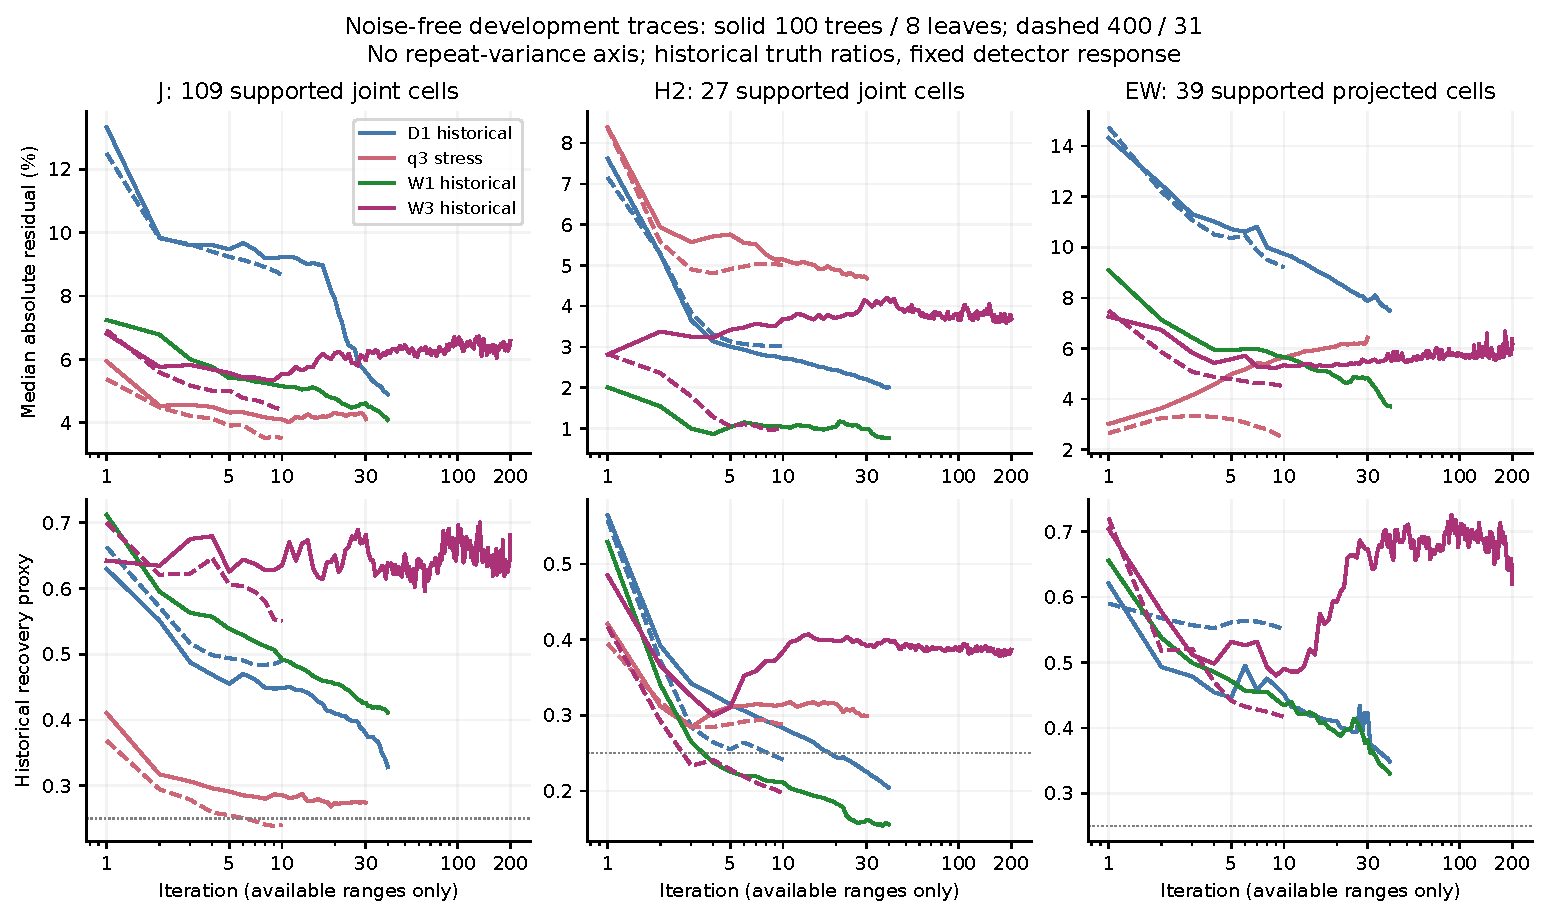
\includegraphics[width=\linewidth]{figures/gbdt_recovery.pdf}

\caption{Noise-free five-dimensional recovery of historical truths at fixed simulated response. Solid curves use 100 trees/8 leaves; dashed use 400/31 for OmniFold estimators. D1 and W1 extend to 40 iterations, $q_3$ stress to 30, W3 to 200, and capacity probes to 10; some baseline traces end at their last saved checkpoint. The upper row gives median $|\hat f/f_{\rm true}-1|$ over supported cells. The lower row gives the study's residual proxy $\operatorname{median}(|\hat f/f_{\rm true}-1|/|f_{\rm true}/f_0-1|)$ for departures above 1\%, with the required bound 0.25 dotted. Different denominators prevent interpreting one minus the proxy as an exact recovered fraction. The $q_3$ stress has no eligible EW departure. These traces measure no repeat variance.}

\label{fig:gbdt-recovery}
\end{figure}

\paragraph{Variability and interval behavior at five iterations.}

Figure~\ref{fig:gbdt-bias-spread} compares ensemble residual means and repeat standard deviations at the same setting. At historical W3 truth, EW29 has mean residual \SI{23.67}{\percent} and repeat SD \SI{0.56}{\percent}; EW7 has \SI{-6.81}{\percent} and \SI{0.30}{\percent}. Small spread does not imply small bias. Coarser cells can have smaller residuals and spread, but they estimate different integrals, so their smaller residuals and spread are not an improvement in precision on an unchanged quantity. No matching repeat ensembles exist at more iterations or larger OmniFold capacity, so no tradeoff can be inferred.

\begin{figure}[tbp]
\centering
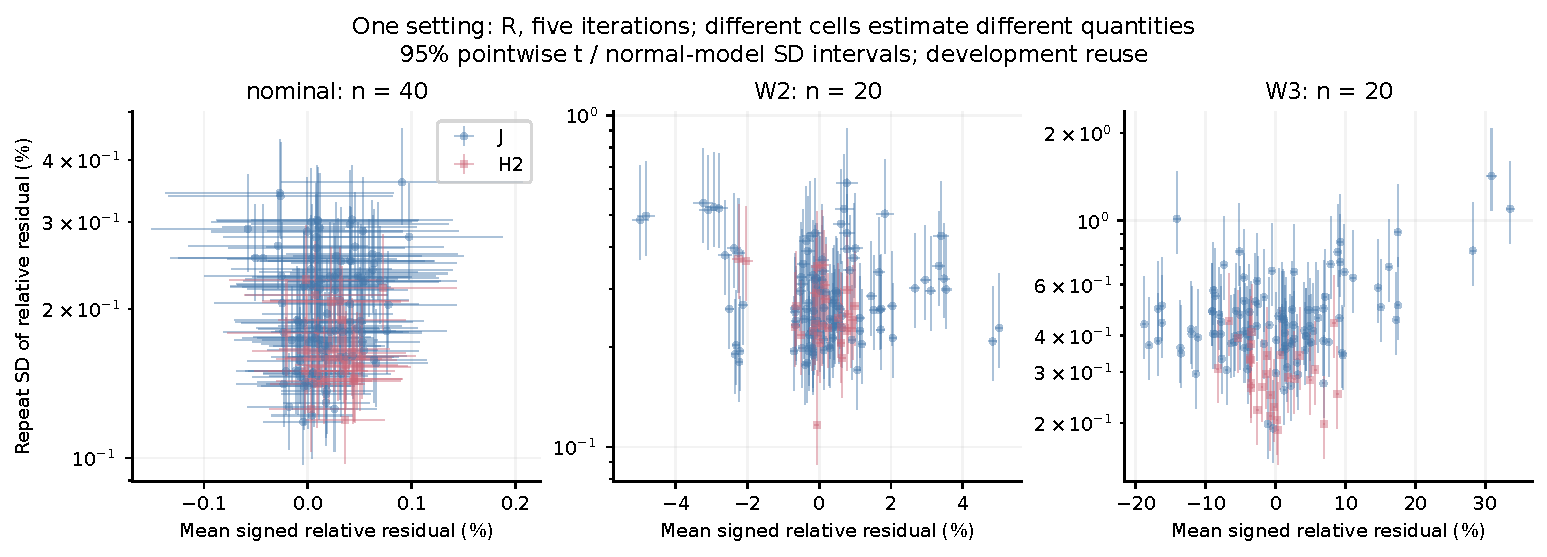
\includegraphics[width=\linewidth]{figures/gbdt_bias_spread.pdf}

\caption{Estimator $R$ at five iterations. Each supported J or H2 cell gives the mean and SD of $(\hat f-f_{\rm true})/f_{\rm true}$ in the same background-inclusive ensemble: 40 nominal experiments, 20 each for W2 and W3. Bars give pointwise 95\% Student-$t$ intervals for means and normal-model intervals for SDs, conditional on saved simulation. They supply neither simultaneous bounds nor total uncertainties. Truth panels and reporting cells form no frontier across estimator settings.}

\label{fig:gbdt-bias-spread}
\end{figure}

The statistical intervals of the development assessment take their width from 100 bootstrap replicas of one nominal development experiment and do not recompute it for each assessment experiment (Fig.~\ref{fig:gbdt-coverage}). At nominal truth, EW41 contains the truth in 15 of 40 68\% intervals (37.5\%, pointwise exact 95\% interval [22.7\%, 54.2\%]), so a pooled pass cannot qualify this cell. A 160-experiment check with the width averaged over six bootstrap estimates changes the pull scales but does not validate the real-data procedure, which uses the data's own width. Finite replica noise explains much of the apparent variation among the six estimates.
% Register round n1 (R-N1): "Neither check establishes total coverage" is covered by the one statement in
% sec:coverage-5d that no frequentist coverage is claimed for any five-dimensional interval.

\begin{figure}[tbp]
\centering
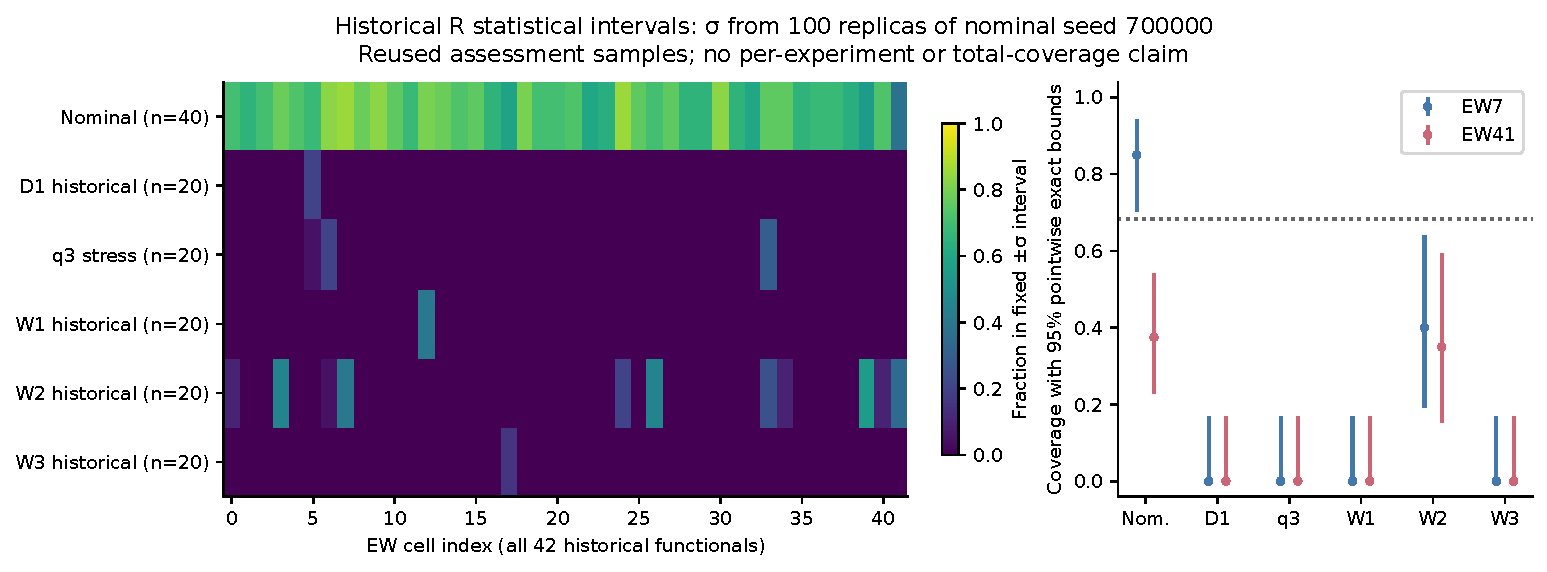
\includegraphics[width=\linewidth]{figures/gbdt_coverage.pdf}

\caption{Development assessment of $R$: containment of the truth in $\hat f\pm\sigma$, with $\sigma$ fixed from the nominal bootstrap, for all 42 EW functionals. Right shows EW7 ($\Eavail\in[0.1,0.2)$, $W\in[1.1,1.4)$ GeV) and EW41 (both above 3 GeV), with pointwise 95\% Clopper--Pearson bounds. The dotted line gives nominal Gaussian 68.27\% coverage. Zero of 20 intervals contain the truth; the upper 95\% bound is 16.8\%, which does not imply zero population coverage. The truth ratios are the historical deformations. No total uncertainty or newly validated interval is shown.}

\label{fig:gbdt-coverage}
\end{figure}

A paired perturbation study supports the containment of rounding variability in the refit-per-replica bootstrap of $R$. Twenty edge-safe data jitters (uniform input perturbations within half a single-precision unit in the last place that keep the fine-grid membership fixed) give a J-cell median SD of \SI{0.228}{\percent}, against a bootstrap SD of \SI{0.368}{\percent}. Fifty bootstrap replicas with jittered partners give a median consistency ratio of 1.02 and an estimated numerical share of 0.37 of the bootstrap variance. In this design, adding the numerical variance to the bootstrap variance would count it twice. The stability failure and the study's scope are in \S\ref{sec:val-departure}, interval coverage in \S\ref{sec:coverage-5d}.

\paragraph{Prior sensitivity is not a measured real-data bias.}

Real-data prior shifts correlate with minus the noise-free residual at the same historical truth (Fig.~\ref{fig:gbdt-prior}). For W3 the correlation over J cells is 0.92, yet $|\mathrm{shift}|\geq|\mathrm{residual}|$ holds in only 71\% of supported J cells (52\% of H2 cells, 54\% of EW cells). Maximum shifts over five historical vertices have medians 12.0\%, 9.6\% and 13.4\% on J, H2 and EW; excluding D1 gives 11.2\%, 4.3\% and 9.9\%. These envelopes are sensitivities: they provide no probabilities, covariance components or guaranteed bias bounds, and the truth of the data has not been shown to lie within their span.

\begin{figure}[tbp]
\centering
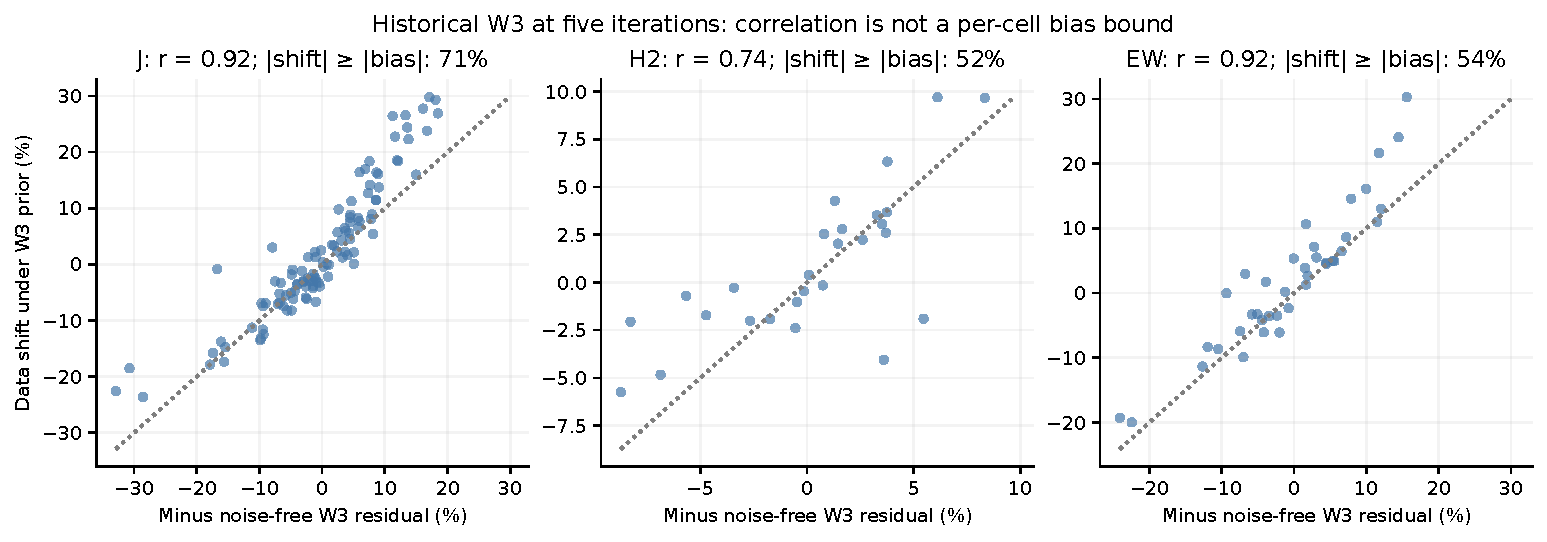
\includegraphics[width=\linewidth]{figures/gbdt_prior_response.pdf}

\caption{Historical W3 at five iterations. Horizontal gives minus the noise-free relative truth residual; vertical gives the relative shift in real-data $R$ when its MC prior changes to W3, normalized to CV-prior results. Points are supported cells, not independent repeated experiments. The diagonal marks equality. Strong correlation supplies no per-cell bound; shifts do not measure unknown real-data bias.}

\label{fig:gbdt-prior}
\end{figure}

Deciding the tradeoff would require sharing pseudo-data and MC splits across a small set of iteration and capacity settings and measuring bias, variance and mean squared error for common functionals. That comparison would not validate intervals, which also requires an explicit treatment of physical nuisances and model dependence. No new ensemble enters these studies.
% Evidence: nd-unfolding/gbdt_model_dependence/{inputs,results,README.md}; VL163.
% Historical grades: s5e A_FAIL; s5p amendment 4 NOT ADMITTED; amendment 6 LOW corrections.

\subsection{Five-dimensional coverage test}
\label{sec:coverage-5d}

An end-to-end independent-truth test assessed statistical intervals of a deterministic five-dimensional estimator variant with nominal-truth bias correction (1,200 pseudo-experiments over three truths). It failed its futility criterion, set before the test was run, at the nominal truth and under a 10\% reduction of the signal rate with a weak $\Eavail$ slope (below). No frequentist coverage is therefore claimed for any five-dimensional interval. Figure~\ref{fig:coverage-5d-paper} shows the coverage of each reported integral under the rate reduction. The intervals divide each estimate by $1+\beta$, where $\beta$ is the relative closure bias at nominal truth, and add the standard error of $\beta$ times the corrected estimate in quadrature to the statistical standard deviation. A quantity fails when the upper confidence bound on its coverage lies below 0.66 for 68\% intervals or below 0.94 for 95\% intervals. The second truth (the $\Eavail$ tilt) multiplies the true signal by $1+0.2\,(\Eavail/\SI{100}{GeV}-\tfrac12)$ without renormalization, with the background unchanged; below $\Eavail=\SI{3}{GeV}$ the weight is 0.900--0.906. Under that change, 51 of the 153 reported cell and projection integrals have 68\% coverage confidently below nominal, with coverage as low as 0.060, and 42 of the 153 fail at 95\%. At nominal truth two of the 153 fail at 95\%, the lowest coverage being 0.850.
% Register round n1 (R-N1, R-N6): the one statement of the five-dimensional interval status, for all of sec:5d;
% "predeclared" (here) and "fixed in advance" (Table tab:validation-design-5d) stated once, as the criterion's timing.
% plain-language pass 2 (DECISION-20261018-joseph-plain-language-pass2): theme A, note home for the paper's
% Sec. IV C numbers. Source: OUTCOME-20260925-s5c-tier-s-futility-fail.md:30-36 (table: nominal 0 / 2 futile,
% min 0.570 / 0.850; E_avail tilt a=0.2 51 / 42 futile, min 0.060 / 0.288; UCB < 0.66 / < 0.94; per-comparison
% level 0.05/459) and :41-43; receipt state/s5c/tier_s/interim_400.json (aa574c17...): 153 functionals =
% 109 J cells + 42 EW cells + the EW all-ones sum + the total integrated rate.
% Methods-paper rewrite draft 5: the interval definition, moved here from the article (nd-unfolding/s5c_coverage.py:77-80).
% Draft 6 (REVIEW-2 finding 13): nd-unfolding/s5c_coverage.py:79-80, half-width z sqrt(sigma^2 + (se f)^2).
% Methods-paper rewrite draft 4 (X5 G5b, verified by the director): nd-unfolding/s5c_pseudo.py:67-70 (weight),
% :125-128 (applied to the pseudo-data signal, not renormalized; background unchanged); KNOWN_ISSUES row 98.

\paragraph{Why the intervals miscover under the rate reduction.} The diagnosis below uses the stored outputs and the code.  The rate change itself is recovered: in the one locally stored pseudo-experiment the total changes by \SI{-9.58}{\percent} against \SI{-9.56}{\percent} injected, and over the 400 the total covers at 0.74 (68\%), so the miscoverage is not a normalization failure.  Nor are the intervals too narrow: they use one nominal bootstrap $\sigma$ at every truth, which for 10\% fewer events is slightly too wide apart from the background not being redrawn (inferred spread about $1.15\sigma$ at $W\ge\SI{3}{GeV}$), and setting the spread equal to the half-width leaves the failing quantities' coverage at 0.06--0.22.  The purity subtraction does not apply a nominal signal fraction to the reduced data: it removes the absolute nominal background expectation, which is unchanged, and in the stored pseudo-experiment the subtracted total agrees with the pseudo-signal to 60 of 3.2 million events.  The miscoverage is a residual bias that the nominal-truth bias correction does not remove.  The rate change adds a positive bias that grows with $W$, about \SI{0.2}{\percent} for $1.4\le W<\SI{2.2}{GeV}$, \SI{0.4}{\percent} for $2.2\le W<\SI{3}{GeV}$, and 0.7--\SI{1.1}{\percent} for $W\ge\SI{3}{GeV}$, which is 1.3--2.6 standard deviations against intervals of 0.16--0.43\%, whatever the sign of the nominal bias $\beta$; removing that bias restores coverage to 0.62--0.82 at 68\% and 0.92--0.99 at 95\%.  These per-quantity biases and spreads are inferred, not measured: the stored output records only hit counts, so each quantity's mean shift and spread come from a Gaussian fit to its 68\% and 95\% coverage, checked against one recorded value (EW17: $+1.04\%$ fitted against $+1.05\%$).  The source of the $W$-graded term is not established: its size and ordering roughly match, under an approximate assignment of background fractions to $W$ bins, the rise of the background fraction by $0.111\,f_{\mathrm{bkg}}$, but the term may also arise from the estimator alone. A rerun of five of the same pseudo-experiments, without background and with the background scaled by 0.9 so that the background-to-signal ratio is restored, did not decide between the two: restoring the ratio raised the residual for $W\ge\SI{3}{GeV}$ rather than removing it, and without background the residual persists.
% Methods-paper rewrite draft 7: docs/orchestration/state/2d-closeout/stageF/methods/M2-RATEFAIL-DIAGNOSIS.md (0 node-h, local receipts and code):
% :8 (total -9.58% recovered against -9.56% injected); :9, :65-69 (spread set equal to the half-width: coverage 0.06-0.22;
% bias removed: 0.62-0.82 at 68%, 0.92-0.99 at 95%); :10, :80-85 (the subtraction removes the nominal absolute
% background expectation, unchanged; the excess is -60 of 3.197M events); :11, :71-76, :100 (W-graded positive residual:
% about +0.2%, +0.4%, +0.7-1.1% for W 1.4-2.2, 2.2-3, >= 3 GeV, 1.3-2.6 sigma against intervals of 0.16-0.43%; added
% whatever the sign of beta); :13, :24 (means and spreads inferred from a Gaussian fit to each 68%/95% coverage pair,
% cross-checked on EW17, +1.04% against +1.05% recorded); :50 (intervals use one nominal bootstrap sigma, slightly too
% wide at 0.9 of the events); :52-63 (failures by W band); :12, :87, :102 (source not established); :15, :104-109
% (confirming test, not run, about 0.1-0.2 node-h).
% 2026-10-22: the test was run (state/ki98-wbias-test/REPORT.md, PR #229; declared and bound before the run), five seeds
% per arm, EW band W >= 3: R_a +2.29 (SE 0.72), R_c +3.40 (0.65), R_b +2.84 (0.46); verdict UNDETERMINED by its rule.

% Source: docs/orchestration/OUTCOME-20260925-s5c-tier-s-futility-fail.md; VALIDATION_LEDGER VL150.

% Register round 2 (2026-10-21): this paragraph's content (376/232/144/121 counts, the uninformative muon projection, the scope, the provenance pointer) merged into the paragraph "Comparison with exact binned unfolding" of sec:val-departure, which now states the diagnostic in full. Note register batch b3 (2026-10-21): the remaining pointer paragraph ("A scoped response-information diagnostic", which only referred to that paragraph) removed.

\subsection{The five-axis covariance of the configuration-(a) central value and its $(\Eavail,W)$ projection}
\label{sec:eavailw-construction}

\paragraph{Status.}
\label{sec:eavailw-adopted}

The five-axis covariance used in this note is the variant centered on the central value (\texttt{cv}); its $(\Eavail,W)$ projection has \zprojCells\ cells. The file and the projection are identified by their SHA-256 checksums (Ref.~\cite{NoteRecords2026}, identities already fixed). The covariance does not meet the acceptance criteria of its specification, and its metadata mark it as not passing and as not to be used. The specification requires the null bound to be fixed before production, which was not done for this covariance, so it cannot meet that requirement. This note nevertheless uses this covariance and its projection. The use does not extend to any other covariance built to the same specification, including the two companion covariances of the measurements below.
% Register round n1 (R-N6): the status stated plainly, once, without "exception" or "the file's own metadata
% records"; the use's scope (this file and projection only) and the two metadata fields are unchanged.
% Deposit pass (DECISION-20261020-joseph-refined-estimator-shorten-delta.md item 2; old text in git history): the file
% name, size and digests move to App. H's identities table; the exception's scope
% (DECISION-20260920-joseph-adopts-z-cv-under-the-6.4-exception.md sec. 3: 3d7465f6... and nothing else, explicitly
% including the two companion products 361090f9... and 7e4636a3...) and the two metadata fields
% (scientific_acceptance, adoptable) are stated as their content.

\paragraph{Construction.} The covariance projects the corrected five-axis statistical covariance as $M C_{5D}M^{\top}$, without rebuilding it in the destination bins, and uses corrected systematic endpoints. Re-selected event loops bound the selection migrations that the single-pass shifted observables omit (\S\ref{sec:uq-higherdim}). On the $\latBins$ reported cells of $(\pT,\pPar,\Eavail,q_{3},W)$, the covariance is

\begin{equation}
  \label{eq:zassembly}
  C_{Z} \;=\; D\,\Big(\textstyle\sum_{V} C_{b}\Big)\,D
  \;+\; \textstyle\sum_{R} C_{b}
  \;+\; \textstyle\sum_{A} L_{b}
  \;+\; C_{\mathrm{stat}}
  \;+\; C_{\mathrm{ML}},
\end{equation}
with the inflation $D=\diag(g)$,
\begin{equation}
  \label{eq:zinflation}
  g_{i} \;=\;
  \sqrt{\frac{\max\!\big(v^{\mathrm{cv}}_{\mathrm{uni},i},\,
                         v_{\mathrm{blk},i}\big)}
             {v_{\mathrm{blk},i}}}
  \;\ge\; 1,
  \qquad
  g_{i}\equiv 1 \ \text{ where } v_{\mathrm{blk},i}=0 .
\end{equation}

Here $v_{\mathrm{blk}}=\diag\big(\sum_{V}C_{b}\big)$ is the vertical block-sum diagonal; $v^{\mathrm{cv}}_{\mathrm{uni}}$ is the unified-throw covariance diagonal \emph{centered on the central value}. Where the denominator is zero, $g=1$ is set by definition, not computed. The band groups $V$ (vertical), $R$ (residual) and $A$ (re-selected lateral) must be disjoint and exhaust the 45 bands. The same inflation of the vertical bands can be transferred onto a sweep block, $\mathbf{C}^{\syst}\!\to\!(\mathbf{C}^{\syst}-\mathbf{C}^{\mathrm{vert}})+\mathbf{G}\,\mathbf{C}^{\mathrm{vert}}\mathbf{G}$ ($\mathbf{G}=\operatorname{diag}g$), only if the low-rank treatment, the mean shift and the selection-support bound above are documented (a condition set in July 2026). This transfer is positive-semidefinite by construction and never falls below the block baseline, whereas a direct rank-$N$ swap is not positive-semidefinite.

\paragraph{Centering, explicitly.} Per-band blocks $C_{b}$ use the MAT-conformant mean-centered $\pm1\sigma$ estimator of \S\ref{app:pair}. Inflation in the CV-centered variant uses $v^{\mathrm{cv}}_{\mathrm{uni}}$. The unified-throw centerings differ by the outer product of measured joint mean shift $\mathbf{ms}$ (joint throw mean minus central value),

\begin{equation}
  \label{eq:zcentering}
  C^{\mathrm{cv}}_{\mathrm{uni}}
  = C^{\mathrm{mean}}_{\mathrm{uni}} + \mathbf{ms}\,\mathbf{ms}^{\top}
  \qquad\Longrightarrow\qquad
  v^{\mathrm{cv}}_{\mathrm{uni},i}-v^{\mathrm{mean}}_{\mathrm{uni},i}
  = \mathbf{ms}_{i}^{2},
\end{equation}

so CV centering retains the mean shift as variance and mean centering removes it. The covariance used here is the CV-centered variant, which retains the shift deliberately; the mean-centered variant (\texttt{mean}) has a $\sqrt{\Tr C}$ lower by \SI{7.13}{\percent}. A file's variant is identified by its metadata, not by its path.

\paragraph{The projection to $(\Eavail,W)$.} The quoted 42-cell covariance is $C_{EW}=M\,C_{Z}\,M^{\top}$, with $M$ of shape $\zprojCells\times\latBins$ over kept axes $(\Eavail,W)$. Each entry of $M$ is the product of the dropped axes' bin widths, giving a differential density in \si{cm^2/GeV^2/nucleon}. Integrating a destination cell requires its own $\Delta\Eavail\,\Delta W$. Rows follow the $7\times6$ $(\Eavail,W)$ grid in measured C order. No source cell is dropped, and the result is exactly symmetric. Support and pinned masks and row-index arrays accompany the covariance and are byte-identical in the two variants. The covariance is paired with the central values of Fig.~\ref{fig:eavailWexcess} by checksum: the central-value array of the projected source and that of the figure are byte-identical, with numerical agreement only as a cross-check.

\paragraph{Conditioning, and why no rank is quoted.} Measured extremes $\lambda_{\min}=+4.359104\times10^{-92}$ and $\lambda_{\max}=1.488215\times10^{-77}$ give $\lambda_{\min}/\lambda_{\max}=2.9\times10^{-15}$ and condition number $\approx3.4\times10^{14}$, at double precision's edge. No eigenvalue is negative, but the smallest lie at the floating-point noise floor of a $\latBins$-term weighted sum. Their sign carries no information: $n_{\mathrm{negative}}=0$ describes this computation and does not show that the source's negative directions were cured. Rank is a property of the cutoff, not of the matrix. The 42 eigenvalues decay smoothly across about fifteen orders of magnitude with no plateau. Retained counts are 26 at relative cutoff $10^{-6}$, 36 at the code default $10^{-12}$, 41 at \texttt{numpy.linalg.matrix\_rank}'s default $n\epsilon=9.3\times10^{-15}$, and 42 without a cutoff. No rank is therefore quoted for this covariance; in particular, 36 is the count at one cutoff, not a number of degrees of freedom. An inverse requires a declared regularization, and none is applied implicitly.

\paragraph{What the covariance supports.}

Four measurements limit what the covariance supports. Items 1, 2 and 4 use two companion covariances built at two estimator-seed settings; only item 3 describes this file.

\begin{enumerate}

\item Estimator-seed sensitivity exceeds its limit. Companion covariances at seed offsets $\{0,1200\}$ give the correlation-sensitive measure $s_{\mathrm{proj}}=\sprojMeasured\,\%$, against the movement limit of \sprojBound\,\%, fixed on 2026-09-18 before production as a direct tolerance at the scale of the ensemble's own precision. A 160-throw ensemble determines a standard deviation only to a relative precision of about $1/\sqrt{2(N-1)}\approx\SI{5.6}{\percent}$ for independent Gaussian throws, so a smaller seed-induced drift could not be resolved against the width it would change. The limit is a declared stability tolerance, not a derived confidence threshold for a maximum over correlated projections. The diagonal-only measures pass ($s_{\mathrm{agg}}=\saggMeasured\,\%$, $s_{\mathrm{med}}=\smedMeasured\,\%$); the failing one probes the off-diagonal structure used by projections.
% Source: docs/orchestration/AUTHORIZATION-20260918-d-resource-required-deliverable-path.md:42 (ruling 5,
% delta = 5% APPROVED; ground: the ~5.6% precision the 160-throw ensemble imposes on sigma).
\item Within the limits stated below, the sensitivity is not the statistic's own resampling noise, which would fall with $N$. With the throw ensemble fixed and only the seed changed, the sensitivity does not fall over the tested ensemble sizes: mean $\seedEffectNforty\,\%$ over four disjoint 40-throw subsets, $\seedEffectNeighty\,\%$ over two 80-throw halves, and $\sprojMeasured\,\%$ over all $N=160$ throws. The same-seed resampling floor falls steeply from $\floorNforty\,\%$ at $N=40$ to $\floorNeighty\,\%$ at $N=80$, with two-point exponent $\floorExponent$; no floor measurement exists at $N=160$. Three limits rule out a statement about infinite ensembles. First, the $40$- and $80$-throw points are nested subsets of the same 160 throws, not independent ensembles. The flatness therefore holds within one ensemble, over a factor of four in $N$; the behaviour at larger $N$ is unmeasured. Second, the quoted $\pm\seedEffectScatter\,\%$ is subset scatter at a single seed pair (offsets $\{0,1200\}$); the width of the distribution over seed pairs is unmeasured. Third, the statistic is a maximum over the declared offset set, so additional pairs can only raise it.
  % Search: floor at N=160; larger ensemble; seed-pair width; seed pairs (values.tex:446 "the FLOOR was measured at N=40 and N=80 ONLY"; nd-unfolding/CORRECTED_UQ_PRODUCTION_STATUS.md:17-22, the 40- and 80-throw points nested in one 160-throw ensemble at one seed pair; CORRECTION-20260921-seed-effect-larger-ensemble-corollary-withdrawn.md:71-74, the N=160 floor of EVIDENCE-20260920 is an extrapolation; release-package-20260922/README.md:35-39, larger N and the seed-pair width unmeasured) @ 624acea1
\item Five of the covariance's 45 bands fall outside the seed variation. The endpoint convention fixes the estimator seed for the muon-energy, muon-resolution and beam-angle blocks, so the offset cannot reach them. They carry $\pinnedBandsSqrtTr\,\%$ of $\sqrt{\mathrm{Tr}\,C}$ and move by exactly zero; their seed sensitivity is unmeasured. Allowing them to vary could move the total in either direction, and neither is measured, because $s_{\mathrm{proj}}$ maximizes relative changes over functionals rather than summing nonnegative component contributions.
\item Seed shifts in central values are a small fraction of their uncertainty. Across the comparison's 43 projection functionals (\zprojCells\ destinations plus the all-ones total rate), shifts reach $\cvMoveProjMax\,\%$, versus relative uncertainties of order ten percent. They reach at most $\cvMoveOverSigmaMax\,\%$ of quoted uncertainty, with median $\cvMoveOverSigmaMed\,\%$. The largest shift occurs in the destination cell driving the covariance result. Individual five-axis bins reach $\cvMoveBinOverSigmaMax\,\%$ of their uncertainty; summing bins suppresses this movement in projections.

\end{enumerate}

\noindent The estimator-seed magnitude criterion specified before production \emph{has not been computed} for this covariance. It was computed only for the two companion covariances built for that purpose, and their outcomes do not transfer to this covariance (Ref.~\cite{NoteRecords2026}, \recentry{z-cv-record}).
% Search: s_proj; M(ii); cause 3; C3; estimator-seed magnitude criterion; z-cv 3d7465f6; GRADE-20260920; VL146; L2 (computed only for 361090f9/7e4636a3, DECISION-20260920-joseph-adopts-z-cv-under-the-6.4-exception.md:36-38; z-cv precursor undeclared so branch 3 unreachable, EVIDENCE-20260919-cause3-member-eligibility-census.md:17-19; later s_proj on other products only, VALIDATION_LEDGER.md:219, OUTCOME-20260922-L2-sproj-measured-and-the-pair-is-not-code-comparable.md:3-5) @ 0d919b1a
